\documentclass[handout]{beamer} % Disable animations
% \documentclass{beamer}
\usefonttheme[onlymath]{serif}
\usetheme{metropolis}
\setbeamertemplate{section in toc}[sections numbered]
\setbeamertemplate{subsection in toc}[subsections numbered]

\usepackage{amsmath}
\usepackage{amsthm}
\usepackage{amssymb}
\usepackage{outlines}
\usepackage{extarrows}
\usepackage{tikz-dependency}
\usepackage{qtree}
\usepackage{bm}
\usepackage[
    type={CC},
    modifier={by-nc},
    version={4.0},
]{doclicense}

% \usepackage{mhchem}
% for \xrightleftharpoons
\usepackage{mathtools}

% \usepackage{lmodern}% http://ctan.org/pkg/lm
% \usepackage{anyfontsize}

\renewcommand\textbullet{\ensuremath{\bullet}}

% Footnote with no number
\newcommand\blfootnote[1]{%
  \begingroup
  \renewcommand\thefootnote{}\footnote{#1}%
  \addtocounter{footnote}{-1}%
  \endgroup
}

\usepackage{setspace}
\usepackage{etoolbox}
\AtBeginEnvironment{quote}{\singlespacing\small}

%%%%% NEW MATH DEFINITIONS %%%%%

% Mark sections of captions for referring to divisions of figures
\newcommand{\figleft}{{\em (Left)}}
\newcommand{\figcenter}{{\em (Center)}}
\newcommand{\figright}{{\em (Right)}}
\newcommand{\figtop}{{\em (Top)}}
\newcommand{\figbottom}{{\em (Bottom)}}
\newcommand{\captiona}{{\em (a)}}
\newcommand{\captionb}{{\em (b)}}
\newcommand{\captionc}{{\em (c)}}
\newcommand{\captiond}{{\em (d)}}

% Highlight a newly defined term
\newcommand{\newterm}[1]{{\bf #1}}


% Figure reference, lower-case.
\def\figref#1{figure~\ref{#1}}
% Figure reference, capital. For start of sentence
\def\Figref#1{Figure~\ref{#1}}
\def\twofigref#1#2{figures \ref{#1} and \ref{#2}}
\def\quadfigref#1#2#3#4{figures \ref{#1}, \ref{#2}, \ref{#3} and \ref{#4}}
% Section reference, lower-case.
\def\secref#1{section~\ref{#1}}
% Section reference, capital.
\def\Secref#1{Section~\ref{#1}}
% Reference to two sections.
\def\twosecrefs#1#2{sections \ref{#1} and \ref{#2}}
% Reference to three sections.
\def\secrefs#1#2#3{sections \ref{#1}, \ref{#2} and \ref{#3}}
% Reference to an equation, lower-case.
\def\eqref#1{equation~\ref{#1}}
% Reference to an equation, upper case
\def\Eqref#1{Equation~\ref{#1}}
% A raw reference to an equation---avoid using if possible
\def\plaineqref#1{\ref{#1}}
% Reference to a chapter, lower-case.
\def\chapref#1{chapter~\ref{#1}}
% Reference to an equation, upper case.
\def\Chapref#1{Chapter~\ref{#1}}
% Reference to a range of chapters
\def\rangechapref#1#2{chapters\ref{#1}--\ref{#2}}
% Reference to an algorithm, lower-case.
\def\algref#1{algorithm~\ref{#1}}
% Reference to an algorithm, upper case.
\def\Algref#1{Algorithm~\ref{#1}}
\def\twoalgref#1#2{algorithms \ref{#1} and \ref{#2}}
\def\Twoalgref#1#2{Algorithms \ref{#1} and \ref{#2}}
% Reference to a part, lower case
\def\partref#1{part~\ref{#1}}
% Reference to a part, upper case
\def\Partref#1{Part~\ref{#1}}
\def\twopartref#1#2{parts \ref{#1} and \ref{#2}}

\def\ceil#1{\lceil #1 \rceil}
\def\floor#1{\lfloor #1 \rfloor}
% \def\1{\bm{1}}
\newcommand{\train}{\mathcal{D}}
\newcommand{\valid}{\mathcal{D_{\mathrm{valid}}}}
\newcommand{\test}{\mathcal{D_{\mathrm{test}}}}

\def\eps{{\epsilon}}


% Random variables
\def\reta{{\textnormal{$\eta$}}}
\def\ra{{\textnormal{a}}}
\def\rb{{\textnormal{b}}}
\def\rc{{\textnormal{c}}}
\def\rd{{\textnormal{d}}}
\def\re{{\textnormal{e}}}
\def\rf{{\textnormal{f}}}
\def\rg{{\textnormal{g}}}
\def\rh{{\textnormal{h}}}
\def\ri{{\textnormal{i}}}
\def\rj{{\textnormal{j}}}
\def\rk{{\textnormal{k}}}
\def\rl{{\textnormal{l}}}
% rm is already a command, just don't name any random variables m
\def\rn{{\textnormal{n}}}
\def\ro{{\textnormal{o}}}
\def\rp{{\textnormal{p}}}
\def\rq{{\textnormal{q}}}
\def\rr{{\textnormal{r}}}
\def\rs{{\textnormal{s}}}
\def\rt{{\textnormal{t}}}
\def\ru{{\textnormal{u}}}
\def\rv{{\textnormal{v}}}
\def\rw{{\textnormal{w}}}
\def\rx{{\textnormal{x}}}
\def\ry{{\textnormal{y}}}
\def\rz{{\textnormal{z}}}

% Random vectors
\def\rvepsilon{{\mathbf{\epsilon}}}
\def\rvtheta{{\mathbf{\theta}}}
\def\rva{{\mathbf{a}}}
\def\rvb{{\mathbf{b}}}
\def\rvc{{\mathbf{c}}}
\def\rvd{{\mathbf{d}}}
\def\rve{{\mathbf{e}}}
\def\rvf{{\mathbf{f}}}
\def\rvg{{\mathbf{g}}}
\def\rvh{{\mathbf{h}}}
\def\rvu{{\mathbf{i}}}
\def\rvj{{\mathbf{j}}}
\def\rvk{{\mathbf{k}}}
\def\rvl{{\mathbf{l}}}
\def\rvm{{\mathbf{m}}}
\def\rvn{{\mathbf{n}}}
\def\rvo{{\mathbf{o}}}
\def\rvp{{\mathbf{p}}}
\def\rvq{{\mathbf{q}}}
\def\rvr{{\mathbf{r}}}
\def\rvs{{\mathbf{s}}}
\def\rvt{{\mathbf{t}}}
\def\rvu{{\mathbf{u}}}
\def\rvv{{\mathbf{v}}}
\def\rvw{{\mathbf{w}}}
\def\rvx{{\mathbf{x}}}
\def\rvy{{\mathbf{y}}}
\def\rvz{{\mathbf{z}}}

% Elements of random vectors
\def\erva{{\textnormal{a}}}
\def\ervb{{\textnormal{b}}}
\def\ervc{{\textnormal{c}}}
\def\ervd{{\textnormal{d}}}
\def\erve{{\textnormal{e}}}
\def\ervf{{\textnormal{f}}}
\def\ervg{{\textnormal{g}}}
\def\ervh{{\textnormal{h}}}
\def\ervi{{\textnormal{i}}}
\def\ervj{{\textnormal{j}}}
\def\ervk{{\textnormal{k}}}
\def\ervl{{\textnormal{l}}}
\def\ervm{{\textnormal{m}}}
\def\ervn{{\textnormal{n}}}
\def\ervo{{\textnormal{o}}}
\def\ervp{{\textnormal{p}}}
\def\ervq{{\textnormal{q}}}
\def\ervr{{\textnormal{r}}}
\def\ervs{{\textnormal{s}}}
\def\ervt{{\textnormal{t}}}
\def\ervu{{\textnormal{u}}}
\def\ervv{{\textnormal{v}}}
\def\ervw{{\textnormal{w}}}
\def\ervx{{\textnormal{x}}}
\def\ervy{{\textnormal{y}}}
\def\ervz{{\textnormal{z}}}

% Random matrices
\def\rmA{{\mathbf{A}}}
\def\rmB{{\mathbf{B}}}
\def\rmC{{\mathbf{C}}}
\def\rmD{{\mathbf{D}}}
\def\rmE{{\mathbf{E}}}
\def\rmF{{\mathbf{F}}}
\def\rmG{{\mathbf{G}}}
\def\rmH{{\mathbf{H}}}
\def\rmI{{\mathbf{I}}}
\def\rmJ{{\mathbf{J}}}
\def\rmK{{\mathbf{K}}}
\def\rmL{{\mathbf{L}}}
\def\rmM{{\mathbf{M}}}
\def\rmN{{\mathbf{N}}}
\def\rmO{{\mathbf{O}}}
\def\rmP{{\mathbf{P}}}
\def\rmQ{{\mathbf{Q}}}
\def\rmR{{\mathbf{R}}}
\def\rmS{{\mathbf{S}}}
\def\rmT{{\mathbf{T}}}
\def\rmU{{\mathbf{U}}}
\def\rmV{{\mathbf{V}}}
\def\rmW{{\mathbf{W}}}
\def\rmX{{\mathbf{X}}}
\def\rmY{{\mathbf{Y}}}
\def\rmZ{{\mathbf{Z}}}

% Elements of random matrices
\def\ermA{{\textnormal{A}}}
\def\ermB{{\textnormal{B}}}
\def\ermC{{\textnormal{C}}}
\def\ermD{{\textnormal{D}}}
\def\ermE{{\textnormal{E}}}
\def\ermF{{\textnormal{F}}}
\def\ermG{{\textnormal{G}}}
\def\ermH{{\textnormal{H}}}
\def\ermI{{\textnormal{I}}}
\def\ermJ{{\textnormal{J}}}
\def\ermK{{\textnormal{K}}}
\def\ermL{{\textnormal{L}}}
\def\ermM{{\textnormal{M}}}
\def\ermN{{\textnormal{N}}}
\def\ermO{{\textnormal{O}}}
\def\ermP{{\textnormal{P}}}
\def\ermQ{{\textnormal{Q}}}
\def\ermR{{\textnormal{R}}}
\def\ermS{{\textnormal{S}}}
\def\ermT{{\textnormal{T}}}
\def\ermU{{\textnormal{U}}}
\def\ermV{{\textnormal{V}}}
\def\ermW{{\textnormal{W}}}
\def\ermX{{\textnormal{X}}}
\def\ermY{{\textnormal{Y}}}
\def\ermZ{{\textnormal{Z}}}

% Vectors
\def\vzero{{\bm{0}}}
\def\vone{{\bm{1}}}
\def\vmu{{\bm{\mu}}}
\def\vtheta{{\bm{\theta}}}
\def\va{{\bm{a}}}
\def\vb{{\bm{b}}}
\def\vc{{\bm{c}}}
\def\vd{{\bm{d}}}
\def\ve{{\bm{e}}}
\def\vf{{\bm{f}}}
\def\vg{{\bm{g}}}
\def\vh{{\bm{h}}}
\def\vi{{\bm{i}}}
\def\vj{{\bm{j}}}
\def\vk{{\bm{k}}}
\def\vl{{\bm{l}}}
\def\vm{{\bm{m}}}
\def\vn{{\bm{n}}}
\def\vo{{\bm{o}}}
\def\vp{{\bm{p}}}
\def\vq{{\bm{q}}}
\def\vr{{\bm{r}}}
\def\vs{{\bm{s}}}
\def\vt{{\bm{t}}}
\def\vu{{\bm{u}}}
\def\vv{{\bm{v}}}
\def\vw{{\bm{w}}}
\def\vx{{\bm{x}}}
\def\vy{{\bm{y}}}
\def\vz{{\bm{z}}}

% Elements of vectors
\def\evalpha{{\alpha}}
\def\evbeta{{\beta}}
\def\evepsilon{{\epsilon}}
\def\evlambda{{\lambda}}
\def\evomega{{\omega}}
\def\evmu{{\mu}}
\def\evpsi{{\psi}}
\def\evsigma{{\sigma}}
\def\evtheta{{\theta}}
\def\eva{{a}}
\def\evb{{b}}
\def\evc{{c}}
\def\evd{{d}}
\def\eve{{e}}
\def\evf{{f}}
\def\evg{{g}}
\def\evh{{h}}
\def\evi{{i}}
\def\evj{{j}}
\def\evk{{k}}
\def\evl{{l}}
\def\evm{{m}}
\def\evn{{n}}
\def\evo{{o}}
\def\evp{{p}}
\def\evq{{q}}
\def\evr{{r}}
\def\evs{{s}}
\def\evt{{t}}
\def\evu{{u}}
\def\evv{{v}}
\def\evw{{w}}
\def\evx{{x}}
\def\evy{{y}}
\def\evz{{z}}

% Matrix
\def\mA{{\bm{A}}}
\def\mB{{\bm{B}}}
\def\mC{{\bm{C}}}
\def\mD{{\bm{D}}}
\def\mE{{\bm{E}}}
\def\mF{{\bm{F}}}
\def\mG{{\bm{G}}}
\def\mH{{\bm{H}}}
\def\mI{{\bm{I}}}
\def\mJ{{\bm{J}}}
\def\mK{{\bm{K}}}
\def\mL{{\bm{L}}}
\def\mM{{\bm{M}}}
\def\mN{{\bm{N}}}
\def\mO{{\bm{O}}}
\def\mP{{\bm{P}}}
\def\mQ{{\bm{Q}}}
\def\mR{{\bm{R}}}
\def\mS{{\bm{S}}}
\def\mT{{\bm{T}}}
\def\mU{{\bm{U}}}
\def\mV{{\bm{V}}}
\def\mW{{\bm{W}}}
\def\mX{{\bm{X}}}
\def\mY{{\bm{Y}}}
\def\mZ{{\bm{Z}}}
\def\mBeta{{\bm{\beta}}}
\def\mPhi{{\bm{\Phi}}}
\def\mLambda{{\bm{\Lambda}}}
\def\mSigma{{\bm{\Sigma}}}

% Tensor
\DeclareMathAlphabet{\mathsfit}{\encodingdefault}{\sfdefault}{m}{sl}
\SetMathAlphabet{\mathsfit}{bold}{\encodingdefault}{\sfdefault}{bx}{n}
\newcommand{\tens}[1]{\bm{\mathsfit{#1}}}
\def\tA{{\tens{A}}}
\def\tB{{\tens{B}}}
\def\tC{{\tens{C}}}
\def\tD{{\tens{D}}}
\def\tE{{\tens{E}}}
\def\tF{{\tens{F}}}
\def\tG{{\tens{G}}}
\def\tH{{\tens{H}}}
\def\tI{{\tens{I}}}
\def\tJ{{\tens{J}}}
\def\tK{{\tens{K}}}
\def\tL{{\tens{L}}}
\def\tM{{\tens{M}}}
\def\tN{{\tens{N}}}
\def\tO{{\tens{O}}}
\def\tP{{\tens{P}}}
\def\tQ{{\tens{Q}}}
\def\tR{{\tens{R}}}
\def\tS{{\tens{S}}}
\def\tT{{\tens{T}}}
\def\tU{{\tens{U}}}
\def\tV{{\tens{V}}}
\def\tW{{\tens{W}}}
\def\tX{{\tens{X}}}
\def\tY{{\tens{Y}}}
\def\tZ{{\tens{Z}}}


% Graph
\def\gA{{\mathcal{A}}}
\def\gB{{\mathcal{B}}}
\def\gC{{\mathcal{C}}}
\def\gD{{\mathcal{D}}}
\def\gE{{\mathcal{E}}}
\def\gF{{\mathcal{F}}}
\def\gG{{\mathcal{G}}}
\def\gH{{\mathcal{H}}}
\def\gI{{\mathcal{I}}}
\def\gJ{{\mathcal{J}}}
\def\gK{{\mathcal{K}}}
\def\gL{{\mathcal{L}}}
\def\gM{{\mathcal{M}}}
\def\gN{{\mathcal{N}}}
\def\gO{{\mathcal{O}}}
\def\gP{{\mathcal{P}}}
\def\gQ{{\mathcal{Q}}}
\def\gR{{\mathcal{R}}}
\def\gS{{\mathcal{S}}}
\def\gT{{\mathcal{T}}}
\def\gU{{\mathcal{U}}}
\def\gV{{\mathcal{V}}}
\def\gW{{\mathcal{W}}}
\def\gX{{\mathcal{X}}}
\def\gY{{\mathcal{Y}}}
\def\gZ{{\mathcal{Z}}}

% Sets
\def\sA{{\mathbb{A}}}
\def\sB{{\mathbb{B}}}
\def\sC{{\mathbb{C}}}
\def\sD{{\mathbb{D}}}
% Don't use a set called E, because this would be the same as our symbol
% for expectation.
\def\sF{{\mathbb{F}}}
\def\sG{{\mathbb{G}}}
\def\sH{{\mathbb{H}}}
\def\sI{{\mathbb{I}}}
\def\sJ{{\mathbb{J}}}
\def\sK{{\mathbb{K}}}
\def\sL{{\mathbb{L}}}
\def\sM{{\mathbb{M}}}
\def\sN{{\mathbb{N}}}
\def\sO{{\mathbb{O}}}
\def\sP{{\mathbb{P}}}
\def\sQ{{\mathbb{Q}}}
\def\sR{{\mathbb{R}}}
\def\sS{{\mathbb{S}}}
\def\sT{{\mathbb{T}}}
\def\sU{{\mathbb{U}}}
\def\sV{{\mathbb{V}}}
\def\sW{{\mathbb{W}}}
\def\sX{{\mathbb{X}}}
\def\sY{{\mathbb{Y}}}
\def\sZ{{\mathbb{Z}}}

% Entries of a matrix
\def\emLambda{{\Lambda}}
\def\emA{{A}}
\def\emB{{B}}
\def\emC{{C}}
\def\emD{{D}}
\def\emE{{E}}
\def\emF{{F}}
\def\emG{{G}}
\def\emH{{H}}
\def\emI{{I}}
\def\emJ{{J}}
\def\emK{{K}}
\def\emL{{L}}
\def\emM{{M}}
\def\emN{{N}}
\def\emO{{O}}
\def\emP{{P}}
\def\emQ{{Q}}
\def\emR{{R}}
\def\emS{{S}}
\def\emT{{T}}
\def\emU{{U}}
\def\emV{{V}}
\def\emW{{W}}
\def\emX{{X}}
\def\emY{{Y}}
\def\emZ{{Z}}
\def\emSigma{{\Sigma}}

% entries of a tensor
% Same font as tensor, without \bm wrapper
\newcommand{\etens}[1]{\mathsfit{#1}}
\def\etLambda{{\etens{\Lambda}}}
\def\etA{{\etens{A}}}
\def\etB{{\etens{B}}}
\def\etC{{\etens{C}}}
\def\etD{{\etens{D}}}
\def\etE{{\etens{E}}}
\def\etF{{\etens{F}}}
\def\etG{{\etens{G}}}
\def\etH{{\etens{H}}}
\def\etI{{\etens{I}}}
\def\etJ{{\etens{J}}}
\def\etK{{\etens{K}}}
\def\etL{{\etens{L}}}
\def\etM{{\etens{M}}}
\def\etN{{\etens{N}}}
\def\etO{{\etens{O}}}
\def\etP{{\etens{P}}}
\def\etQ{{\etens{Q}}}
\def\etR{{\etens{R}}}
\def\etS{{\etens{S}}}
\def\etT{{\etens{T}}}
\def\etU{{\etens{U}}}
\def\etV{{\etens{V}}}
\def\etW{{\etens{W}}}
\def\etX{{\etens{X}}}
\def\etY{{\etens{Y}}}
\def\etZ{{\etens{Z}}}

% The true underlying data generating distribution
\newcommand{\pdata}{p_{\rm{data}}}
% The empirical distribution defined by the training set
\newcommand{\ptrain}{\hat{p}_{\rm{data}}}
\newcommand{\Ptrain}{\hat{P}_{\rm{data}}}
% The model distribution
\newcommand{\pmodel}{p_{\rm{model}}}
\newcommand{\Pmodel}{P_{\rm{model}}}
\newcommand{\ptildemodel}{\tilde{p}_{\rm{model}}}
% Stochastic autoencoder distributions
\newcommand{\pencode}{p_{\rm{encoder}}}
\newcommand{\pdecode}{p_{\rm{decoder}}}
\newcommand{\precons}{p_{\rm{reconstruct}}}

\newcommand{\laplace}{\mathrm{Laplace}} % Laplace distribution

\newcommand{\E}{\mathbb{E}}
\newcommand{\Ls}{\mathcal{L}}
\newcommand{\R}{\mathbb{R}}
\newcommand{\emp}{\tilde{p}}
\newcommand{\lr}{\alpha}
\newcommand{\reg}{\lambda}
\newcommand{\rect}{\mathrm{rectifier}}
\newcommand{\softmax}{\mathrm{softmax}}
\newcommand{\sigmoid}{\sigma}
\newcommand{\softplus}{\zeta}
\newcommand{\KL}{D_{\mathrm{KL}}}
\newcommand{\Var}{\mathrm{Var}}
\newcommand{\standarderror}{\mathrm{SE}}
\newcommand{\Cov}{\mathrm{Cov}}
% Wolfram Mathworld says $L^2$ is for function spaces and $\ell^2$ is for vectors
% But then they seem to use $L^2$ for vectors throughout the site, and so does
% wikipedia.
\newcommand{\normlzero}{L^0}
\newcommand{\normlone}{L^1}
\newcommand{\normltwo}{L^2}
\newcommand{\normlp}{L^p}
\newcommand{\normmax}{L^\infty}

\newcommand{\parents}{Pa} % See usage in notation.tex. Chosen to match Daphne's book.

\DeclareMathOperator*{\argmax}{arg\,max}
\DeclareMathOperator*{\argmin}{arg\,min}

\DeclareMathOperator{\sign}{sign}
\DeclareMathOperator{\Tr}{Tr}
\let\ab\allowbreak


% No footnote separator
% \renewcommand*\footnoterule{}


\title{\textbf{NLP Paper Reading 1}:\\
A Unified Architecture for Natural Language
Processing: Deep Neural Networks with Multitask Learning (2008)}

% \date{\today}
\date{February 2, 2019}
\author{Jorge Balazs}
\institute{\doclicenseImage[imagewidth=4em]}
% \institute{}

% \AtBeginSection[]{%
%   \begin{frame}
%     \frametitle{Contents}
%     \tableofcontents[currentsection]
%   \end{frame}
% }

\begin{document}
  \maketitle

  % \begin{frame}{Contents}
  %   \tableofcontents
  % \end{frame}

  % \section{Introduction}
  % \section{NLP Tasks}
  % \section{General Deep Architecture for NLP}
  %   \subsection{Transforming Indices into Vectors}
  %   \subsection{Variable Sentence Length}
  %   \subsection{Deep Architecture}
  %   \subsection{Related Architectures}
  % \section{Multitasking with Deep NN}
  %   \subsection{Deep Joint Training}
  %   \subsection{Previous Work in MLT for NLP}
  % \section{Leveraging Unlabeled Data}
  % \section{Experiments}
  % \section{Conclusion}

  \section{Paper Structure}
  \begin{frame}{Paper Structure}
      \begin{outline}[enumerate]
        \1[] Abstract
        \1 Introduction
        \1 NLP Tasks
        \1 General Deep Architecture for NLP
          \2 Transforming Indices into Vectors
          \2 Variable Sentence Length
          \2 Deep Architecture
          \2 Related Architectures
        \1 Multitasking with Deep NN
          \2 Deep Joint Training
          \2 Previous Work in MLT for NLP
        \1 Leveraging Unlabeled Data
        \1 Experiments
        \1 Conclusion
      \end{outline}
  \end{frame}

  \section{Abstract}
  \begin{frame}{Abstract}
      \textbf{What}:
      \begin{itemize}
          \item Show that both \textit{multitask learning} (MTL) and
              \textit{semi-supervised learning} improve the generalization of
              shared tasks.
      \end{itemize}
      \textbf{How}:
      \begin{itemize}
          \item Network is trained \textit{jointly} on several NLP tasks.
          \item Sentence $\xlongrightarrow{\text{input}}$ CNN Architecture
              $\xlongrightarrow{\text{output}}$ host of NLP predictions.

      \end{itemize}
  \end{frame}


  \section{Introduction}
  \begin{frame}{Introduction - Background}
      \begin{itemize}[<+->]
          \item NLP = human language $\xlongrightarrow{}$ formal representation
              understandable by computers.
          \item Some applications: information extraction, machine translation,
              summarization, search, human-computer interfaces.
             \pause[\thebeamerpauses]\color{gray}Can you think of any others?
             \pause%

          \item Semantic understanding still is a far distant goal.
              \pause[\thebeamerpauses]{\color{gray}This is still true today.}
              \pause%

              \begin{itemize}
                  \item[] NLP is usually addressed by solving several
                    \textit{syntactic} and \textit{semantic} subtasks (eg, POS
                    tagging, syntactic parsing, and semantic-role labeling).
              \end{itemize}

          \item It is common to analyze these tasks separately.

      \end{itemize}
  \end{frame}

  \begin{frame}{Introduction - Current Limitations}
      \begin{itemize}[<+->]
          \item Common failings of current approaches
              \begin{enumerate}
                  \item They are shallow, ie classifiers are linear.\pause[\thebeamerpauses]
                      {\color{gray}What does this mean?}\pause%
                  \item Linear classifiers need good hand-engineered
                      features. \pause[\thebeamerpauses]{\color{gray}Why is
                      this not desirable?}\pause%
                  \item Features learned in different tasks are
                      \textit{cascaded}, which propagates errors.
              \end{enumerate}

      \end{itemize}
  \end{frame}

  \begin{frame}{Introduction - Proposal}
      A unified architecture that \textit{learns features} relevant to the tasks
      at hand, with little prior knowledge.\pause%

        \textbf{How?}\pause%

    By \textit{jointly} training a Deep Neural Network for solving several NLP
    tasks.\pause%

    {\footnotesize\color{gray}The language model is an exception; we'll talk about this
    later.}

  \end{frame}

  \begin{frame}{Introduction - Contributions}
      They show that:
      \begin{itemize}[<+->]
          \item Multitask learning and semi-supervised learning significantly
              improve performance of Semantic-role labeling, \textit{without
              hand-engineered features}.
          \item Combined tasks (MTL), and the unsupervised task (Language
              Model), learn features that encode semantic information with no
              other supervision than the labeled data from the tasks.
          
      \end{itemize}

 \pause{}{\footnotesize\color{gray}Does this sound familiar? Remember this paper
 was written more than 8 years ago, before AlexNet in 2012 and before the Deep
 Learning wave.}

  \end{frame}


  \section{NLP Tasks}
  \begin{frame}{Part-of-Speech Tagging (POS)}

      \begin{center}
          $\underset{\texttt{JJ}}{\text{Colorless}}$
          $\underset{\texttt{JJ}}{\text{green}}$
          $\underset{\texttt{NNS}}{\text{ideas}}$
          $\underset{\texttt{VBP}}{\text{sleep}}$
          $\underset{\texttt{RB}}{\text{furiously}}$
      \end{center}
      
  \end{frame}

  \begin{frame}{Chunking}
      \begin{center}
        \hspace{-2.7cm}
        \Tree[.S
        [.NP [.\texttt{JJ} Colorless ] [.\texttt{JJ} green ] [.\texttt{NNS} ideas ]]
        [.VP [.\texttt{VBP} sleep ]
        [.ADVP [.\texttt{RB} furiously ]]]
        [.. . ]]
      \end{center}
  \end{frame}

  \begin{frame}{Named Entity Recognition (NER)}
      \begin{center}
          $\underset{\text{PERSON}}{\text{Donal Trump}}$
          joined
          $\underset{\text{ORG}}{\text{Google}}$
          as a researcher
          $\underset{\text{DATE}}{\text{last monday}}$
      \end{center}
  \end{frame}

  \begin{frame}{Semantic Role Labeling (SRL)}
    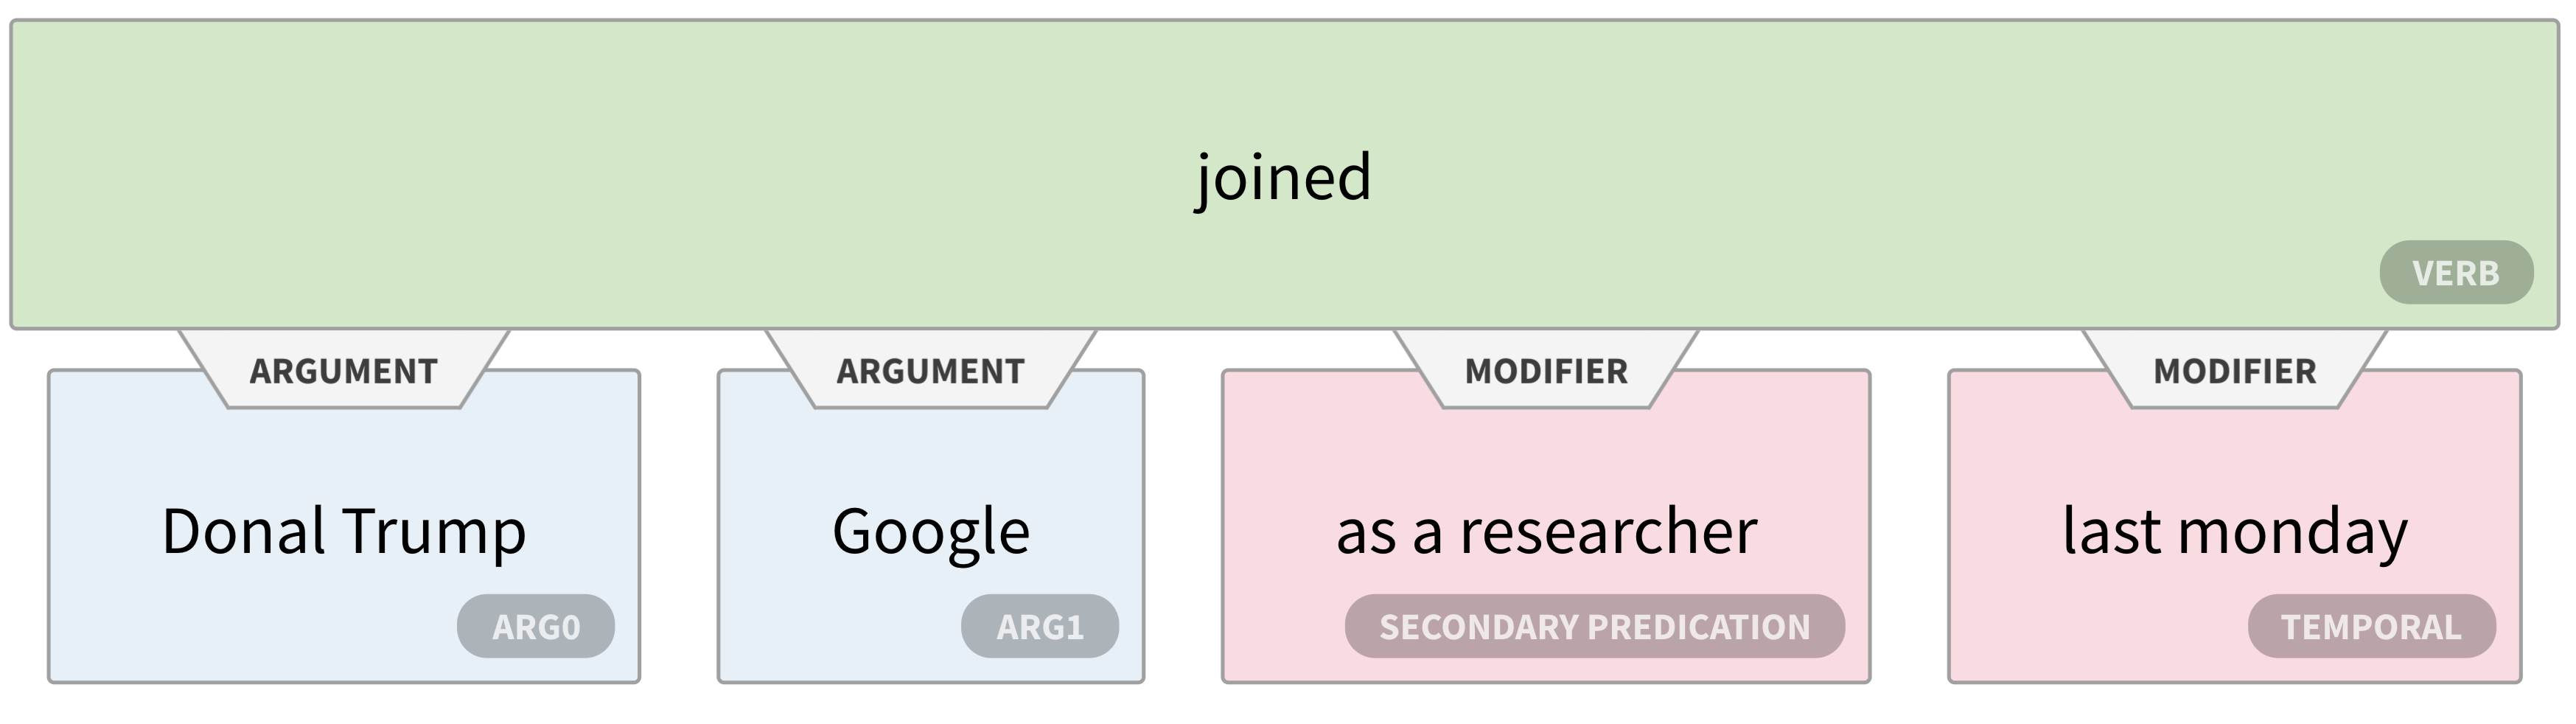
\includegraphics[width=\textwidth]{imgs/SRL.png}
    \blfootnote{\color{gray}\tiny\url{https://demo.allennlp.org/semantic-role-labeling/NTc2MzE2}}
  \end{frame}

  \begin{frame}{Language Models}
      Predict the next word, given the previous words.
   \begin{quote}
     Language modeling is the task of assigning a probability to sentences in a
     language [...]. Besides assigning a probability to each sequence of words, the
     language models also assigns a probability for the likelihood of a given word
     (or a sequence of words) to follow a sequence of words [...]
     \cite{goldberg2017neural}.
   \end{quote}  
  \end{frame}

  \begin{frame}{Semantically Related Words}
      Predicting whether two words are semantically related:
      \begin{itemize}
          \item Mammal $\xrightleftharpoons[HYPONYM]{HYPERNYM}$ Cat
              \vspace{0.5cm}
          \item Car $\xrightleftharpoons[MERONYM]{HOLONYM}$ Wheel
              \vspace{0.5cm}
          \item PC $\xlongleftrightarrow{SYNONYM}$ Computer
    \end{itemize}
  \end{frame}


  \section{General Deep Architecture for NLP}
  \begin{frame}{General Deep Architecture for NLP - Traditional Approaches}
      \begin{itemize}[<+->]

         \item The previous tasks can all be seen as assigning labels to words.
         \item The common approach is to manually transform input sentences into
             vectors (feature engineering), and feed these vectors to a shallow
             classifier (eg, SVM).
         \item The choice of features (feature engineering), is an empirical
             process dependent on the task at hand, mainly based on trial and
             error, and difficult to scale.

      \end{itemize}
  \end{frame}


  \begin{frame}{General Deep Architecture for NLP - Proposed Approach}
      \begin{itemize}[<+->]

          \item They propose a Deep Neural Network (NN) trained in an end-to-end
              fashion.
          \item Features (intermediate representations between the input and
              output) are \textit{learned automatically} by the NN.

      \end{itemize}
  \end{frame}

  \begin{frame}{General Deep Architecture for NLP - Proposed Approach}
      \begin{center}
          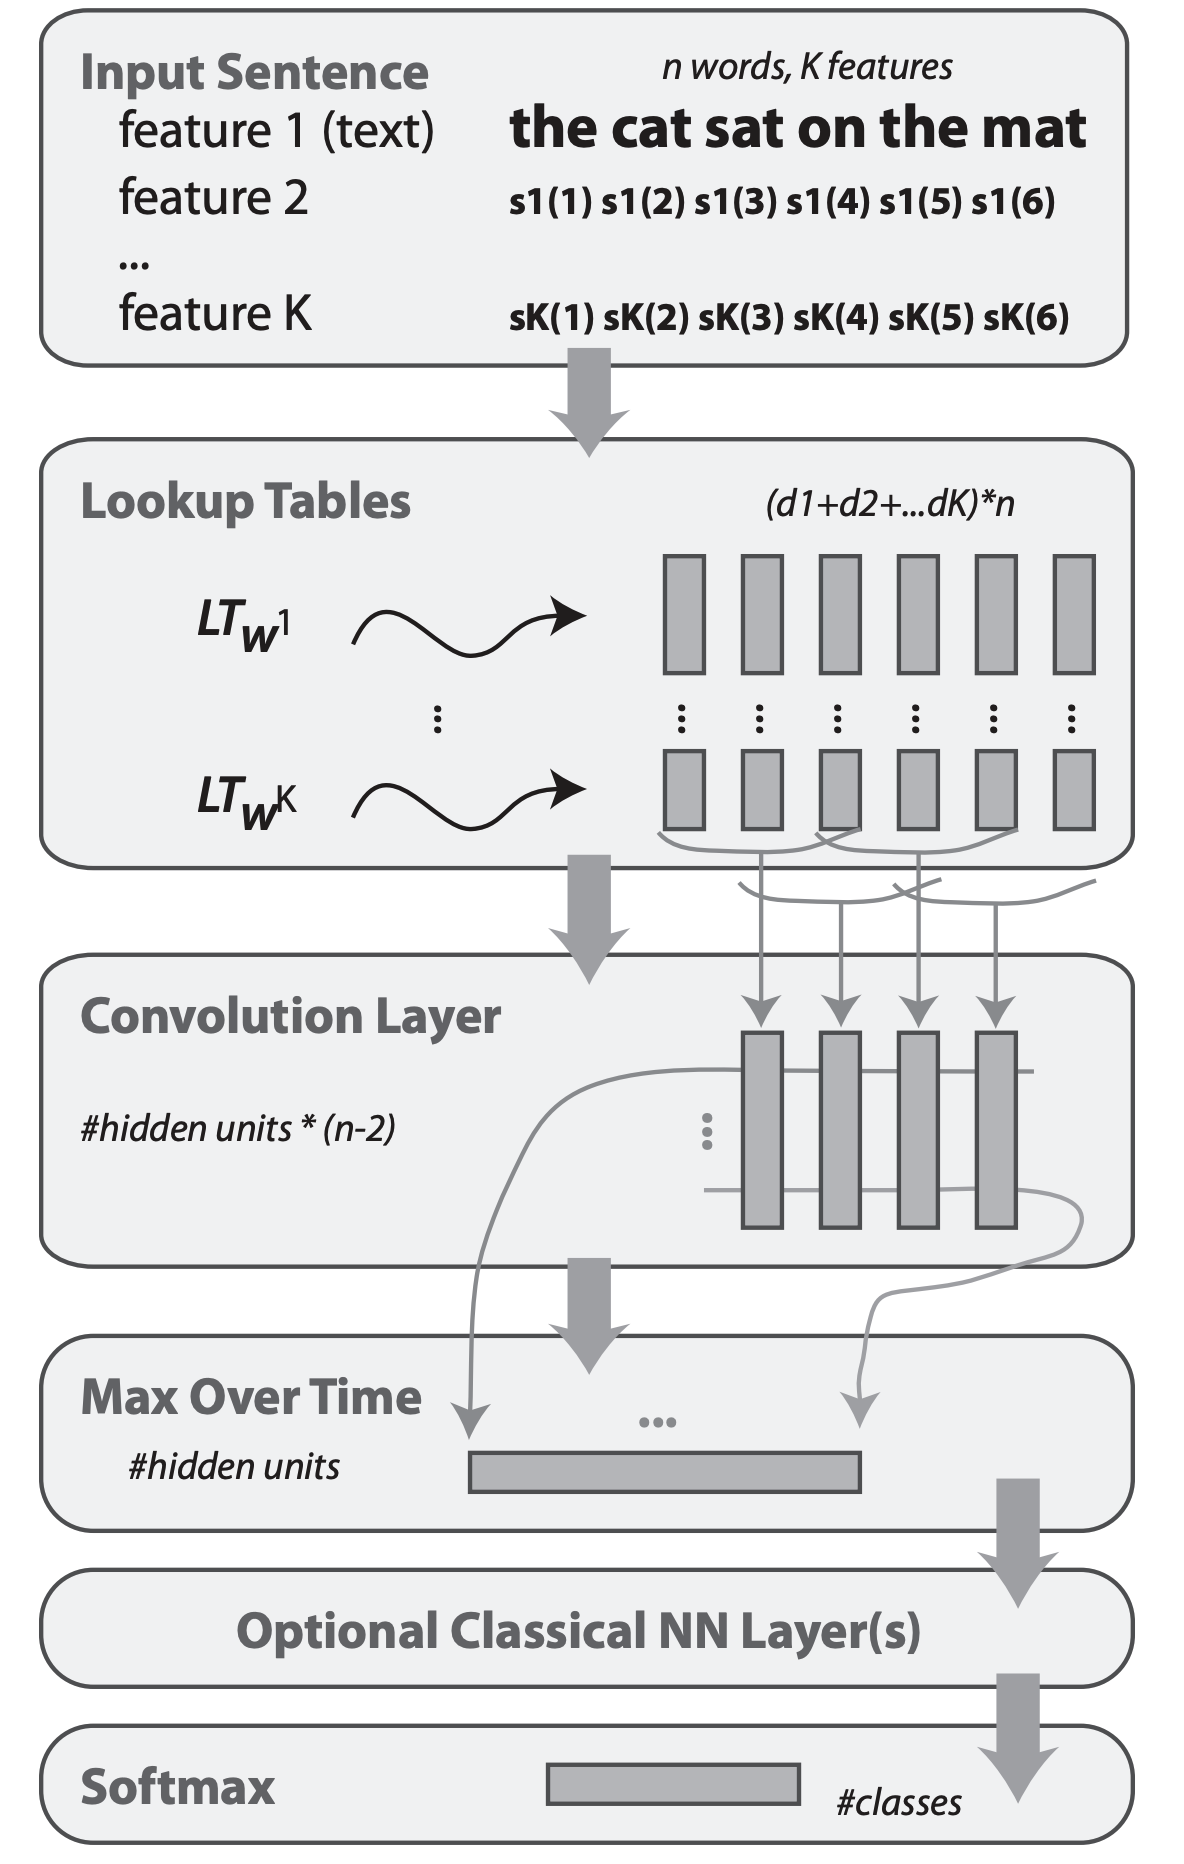
\includegraphics[scale=0.25]{imgs/Architecture.png}
      \end{center}
  \end{frame}

  \begin{frame}{General Deep Architecture for NLP - Transforming Indices into Vectors}
      \begin{itemize}[<+->]
          \item They assume a mapping between words and a set of indices
              $\mathcal{D}$ which is a subset of the Natural numbers
              ($\mathcal{D}\subset\mathbb{N}$).
              \begin{itemize}
                  \item $|\mathcal{D}|$ is the number of elements in
                      $\mathcal{D}$, ie the words we ``know'' (words
                      that appear in the training set).
                  \item $\mathcal{D} = \{1, 2, \ldots, |\mathcal{D}|\}$
              \end{itemize}
      \end{itemize}
  \end{frame}

  \begin{frame}{General Deep Architecture for NLP - Transforming Indices into Vectors}
       \begin{itemize}[<+->]
          \item They also define the relationship between these indices and an
              \textit{embedding lookup table}.
              \begin{itemize}

                  \item This lookup table is simply a matrix $\mW$ where each column
                     corresponds to a vector of dimension $d$ that represents
                     one of the indices in $\mathcal{D}$. Therefore $\mW$
                     has $d$ rows and $|\mathcal{D}|$ columns, and since it
                     contains only real numbers we say that
                     $\mW\in\sR^{d\times|\mathcal{D}|}$.
                  \item $LT_W(i)$ is a function that takes an index $i$ in
                      $\mathcal{D}$ as input, and returns the $i$-th column of
                      $\mW$; a vector $\mW_i$ of dimension $d$ ($\mW_i\in\sR^d$).
                 \item These vectors are learned during training.
              \end{itemize}

      \end{itemize}
  \end{frame}

  \begin{frame}{General Deep Architecture for NLP - Transforming Indices into Vectors}
       \begin{itemize}[<+->]
          \item In general, we can have mappings between any kind of word-level
              feature and a set of indices.
              \begin{itemize}
                  \item For example, capitalization of words is a feature.
                      Our ``vocabulary'' of capitalization features is
                      $\mathcal{D}^{cap}=\{1, 2\}$, where $1$ corresponds to
                      non-capitalized and $2$ to capitalized.
                 \item Similar to the embedding lookup table $\mW$ mentioned
                     previously, we can define $\mW^{cap}\in\sR^{m\times
                         2}$.\footnote[frame]{$m$ is the dimensionality we chose for these
                     specific vectors, and $|\mathcal{D}^{cap}|=2$. Also
                 note that $m$ does not necessarily equal $d$.}
                 \item Equivalently, we will also have a mapping between the
                     elements in $\mathcal{D}^{cap}$ and $\mW^{cap}$ given by
                     $LT_{W^{cap}}(i)=\mW^{cap}_{i}$.
              \end{itemize}

      \end{itemize}
     
  \end{frame}

  \begin{frame}{General Deep Architecture for NLP - Transforming Indices into Vectors}
       \begin{itemize}[<+->]

         \item For each word, we will have several word-level features. For each of
         these features we will have a single vector.
     \item The representation of each word, will be the \textit{concatenation} of these
           vectors.
         \item For example, if we only consider the words themselves and their
             capitalization (see previous slides), each word will be represented
             by a vector $\in\sR^{m+d}$.
      \end{itemize}
  \end{frame}

  \begin{frame}{General Deep Architecture for NLP - Variable Sentence Length}
       \begin{itemize}[<+->]
           \item Let's assume that we have a sequence $\{s_1, \ldots, s_n\}$ of
               $n$ words, each with a corresponding vector
               $\{\vx_1,\ldots,\vx_n\}$ obtained through the
               procedure described earlier.
           \item Each $\vx_i$ will have the same dimension, say
               $d$, ie $\vx_i\in\sR^d$.\footnote[frame]{Not the
               same $d$ mentioned earlier; just a redefinition.}
           \item Clearly the number of vectors we end up with, $n$, depends on 
               the length of the original sentence, however
               NNs know only how to deal with fixed-length inputs.
           % \item The solution the authors propose is to use a \textit{window
           %     approach}. \pause%
           %     {\color{gray}Actually this approach doesn't solve the
           %     variable-length problem. What it does is to incorporate
           %     neighborhood information into the vector representation of each
           %     word.}
      \end{itemize}
      \begin{center}
          \pause[\thebeamerpauses]How do we solve this problem?
      \end{center}
  \end{frame}

  \begin{frame}{General Deep Architecture for NLP - Variable Sentence Length}
      \begin{itemize}[<+->]
          \item A simple approach is to use \textit{window approach} with a
              window size of $ksz$. \pause[\thebeamerpauses]{\color{gray}What
              exactly do they mean by a window approach?}
          \item This approach works well for modeling local phenomena, which
                  is beneficial for tasks such as POS tagging.
          \item It fails, however, when modeling long-range dependencies, which
              is required for more complex tasks such as SRL.
      \end{itemize}

 \pause[\thebeamerpauses]{\color{gray}Why is it ok to model local phenomena in
 POS tagging but not in SRL?}

  \end{frame}

  \begin{frame}{General Deep Architecture for NLP - Variable Sentence Length}
      \begin{itemize}[<+->]
          \item An alternative approach is to use Time-Delay Neural Networks
              (roughly equivalent to CNNs), which are capable of modeling
              long-range dependencies.
            \item $\vo(t)=\sum_{j=1-t}^{n-t}{\mL_j \cdot \vx_{t+j}}$, where
                $\mL_j\in\sR^{n_{hu}\times d}$. Remember that our word vectors
                $\vx_t\in\sR^d$, which means that $\vo(t)\in\sR^{n_{hu}}$ for
                every $t$.

      \end{itemize}

  \end{frame}

  \begin{frame}{General Deep Architecture for NLP - Variable Sentence Length}
      \begin{centering}
          \vspace{-1.8cm}
          $$\vo(t)=\sum_{j=1-t}^{n-t}{\mL_j \cdot \vx_{t+j}}$$
          \vspace{-0.5cm}
          \begin{itemize}[<+->]
              % \item[] $\vo(0)=\sum_{j=1}^{n}{\mL_j\cdot\vx_{0+j}}=\mL_1\vx_1+\mL_2\vx_2+\ldots+\mL_n\vx_n$
              \item[] $\vo(1)=\sum_{j=0}^{n-1}{\mL_j\cdot\vx_{1+j}}=\mL_0\vx_1+\mL_1\vx_2+\ldots+\mL_{n-1}\vx_n$
              \item[] $\vo(2)=\sum_{j=-1}^{n-2}{\mL_j\cdot\vx_{2+j}}=\mL_{-1}\vx_1+\mL_0\vx_2+\ldots+\mL_{n-2}\vx_n$
              \item[] \hspace{5cm}\vdots
              \item[] $\vo(t)=\sum_{j=1-t}^{n-t}{\mL_j\cdot\vx_{t+j}}=\mL_{1-t}\vx_1+\mL_{2-t}\vx_2+\ldots+\mL_{n-t}\vx_n$
              \item[] \hspace{5cm}\vdots
              \item[] $\vo(n)=\sum_{j=1-n}^{0}{\mL_j\cdot\vx_{n+j}}=\mL_{1-n}\vx_1+\mL_{2-n}\vx_2+\ldots+\mL_{0}\vx_n$

      \end{itemize}
          
      \end{centering}

  \end{frame}

  \begin{frame}{General Deep Architecture for NLP - Variable Sentence Length}

    Let's call the window size $w$, i.e., $w=ksz$. We impose
    $\mL_j=\bm{0}\enspace$ if $|j|>\frac{(w-1)}{2}$, or, in other words, $\mL_j$
    will be non-zero iff
    
    $$\enspace-\frac{(w-1)}{2} \leq j \leq \frac{(w-1)}{2}$$

    \pause Let's set $w=3$, i.e., $\mL_j\neq\bm{0}\enspace$
    if $\enspace-1 \leq j \leq 1$

    \pause Our convolution operation becomes:
    $$\vo(t)=\sum_{-1 \leq j \leq 1}{\mL_j \cdot \vx_{t+j}}$$

    \pause Which means that each sum will have only $w=3$ elements.

  \end{frame}

  \begin{frame}{General Deep Architecture for NLP - Variable Sentence Length}

    $$\vo(t)=\sum_{-1 \leq j \leq 1}{\mL_j \cdot \vx_{t+j}}$$

      \begin{centering}
          \begin{itemize}[<+->]
              % \item[] $\vo(0)=\mL_{-1}\vx_{-1}+\mL_0\vx_0+\mL_1\vx_1$
              \item[] $\vo(1)=\mL_{-1}\vx_{0}+\mL_0\vx_{1}+\mL_1\vx_2$
              \item[] $\vo(2)=\mL_{-1}\vx_{1}+\mL_0\vx_{2}+\mL_1\vx_3$
              \item[] \hspace{2.7cm}\vdots
              \item[] $\vo(t)=\mL_{-1}\vx_{t-1}+\mL_0\vx_{t}+\mL_1\vx_{t+1}$
              \item[] \hspace{2.7cm}\vdots
              \item[] $\vo(n-1)=\mL_{-1}\vx_{n-2}+\mL_0\vx_{n-1}+\mL_1\vx_{n}$
              \item[] $\vo(n)=\mL_{-1}\vx_{n-1}+\mL_0\vx_{n}+\mL_1\vx_{n+1}$
         \end{itemize}
      \end{centering}
  \end{frame}


  \begin{frame}{General Deep Architecture for NLP - Variable Sentence Length}
      \begin{itemize}[<+->]
          \item Before the TDNN we had $n$ word vectors
           $\{\vx_1,\ldots,\vx_n\},\enspace\vx_t\in\sR^d$; one for each word of
           our sequence, obtained from a lookup embedding table.
       \item After the TDNN, we have $n$ vectors $\{\vo_1,\ldots,\vo_n\},
           \enspace\vo_t\in\sR^{n_{hu}}$, still one for each word of our
           sequence, where each $\vo_t$ encodes a notion of its
           neighborhood.
       \item Also note that the previous statement is true independently of the
           window size we chose.
       \item This allows to easily pass the output to the first TDNN to another
           TDNN with different parameters and maybe a different window size
           (what the authors refer to as \textit{stacking}).

        
      \end{itemize}
  \end{frame}

  \begin{frame}{General Deep Architecture for NLP - Variable Sentence Length}
      \begin{itemize}[<+->]

        \item After the previous steps we still have $n$ vectors though.
            To obtain a single vector for representing the sentence the authors
            use a ``Max'' Layer (aka maxpooling), over the sequence dimension.
        \item The maxpooling operation reduces the sequence dimension and
            returns a single vector $\vo\in\sR^{n_{hu}}$ representing the whole
            sentence.
        \item This sentence representation can then be passed to a Feedforward
            (aka dense) NN layer.
          \item Finally, they encode the position of the word to be labelled
              with an additional lookup table $LT^{dist_w}(i-pos_w)$.
      \end{itemize}
  \end{frame}

  \begin{frame}{General Deep Architecture for NLP - Deep Architecture}
      \begin{itemize}[<+->]
          \item This part describes how they transform the maxpooled output of
              the TDNN $\vo\in\sR^{n_{hu}}$ into a vector $\vo^{last}\in\sR^k$
              where $k$ is the number of classes in the NLP classification task,
              for example, the number of possible POS tags.
          \item Finally, $\vo^{last}\in\sR^k$ is fed to a softmax layer, which
              returns a vector representing a probability distribution over the
              possible classes: $\vp\in\sR^k$, where $0\leq\vp_i\leq1$ and
              $\sum_{i=1}^k{\vp_i}=1$
      \end{itemize}
  \end{frame}

  \section{Multitasking with Deep NN}

  \begin{frame}{Multitasking with Deep NN}
  \begin{quote}
    Multitask learning is the procedure of learning several tasks at the same
    time with the aim of mutual benefit.
  \end{quote}

  % \begin{center}
  %     \pause{\color{gray}How can doing this benefit the learning procedure?}
  % \end{center}
  \end{frame}

  \begin{frame}{Multitasking with Deep NN - Deep joint Training}
      \begin{itemize}[<+->]
          \item The benefit comes from learning features (representations) that
              are beneficial for several tasks (\textit{more general} features).
          \item Usually, POS predictions are often used for solving
              the NER and SRL tasks. Having good representations for POS
              tagging, might improve both NER and SRL.
          \item Earliest layers (lookup tables) implicitly learn relevant word
              representations for each word. It's reasonable to expect that
              these features will perform well in related tasks.
          \item Earlier layers can be shared accross tasks while later ones can
              be task-specific.
      \end{itemize}
      
  \end{frame}

  \begin{frame}{Multitasking with Deep NN - Deep joint Training}
      \begin{itemize}[<+->]
          \item Their model is trained one example at a time.
          \item At each iteration
              they pick a random example from a random task, feed it forward,
              obtain the loss, calculate the gradients, and backpropagate them.
      \end{itemize}

      \begin{center}
        \pause[\thebeamerpauses]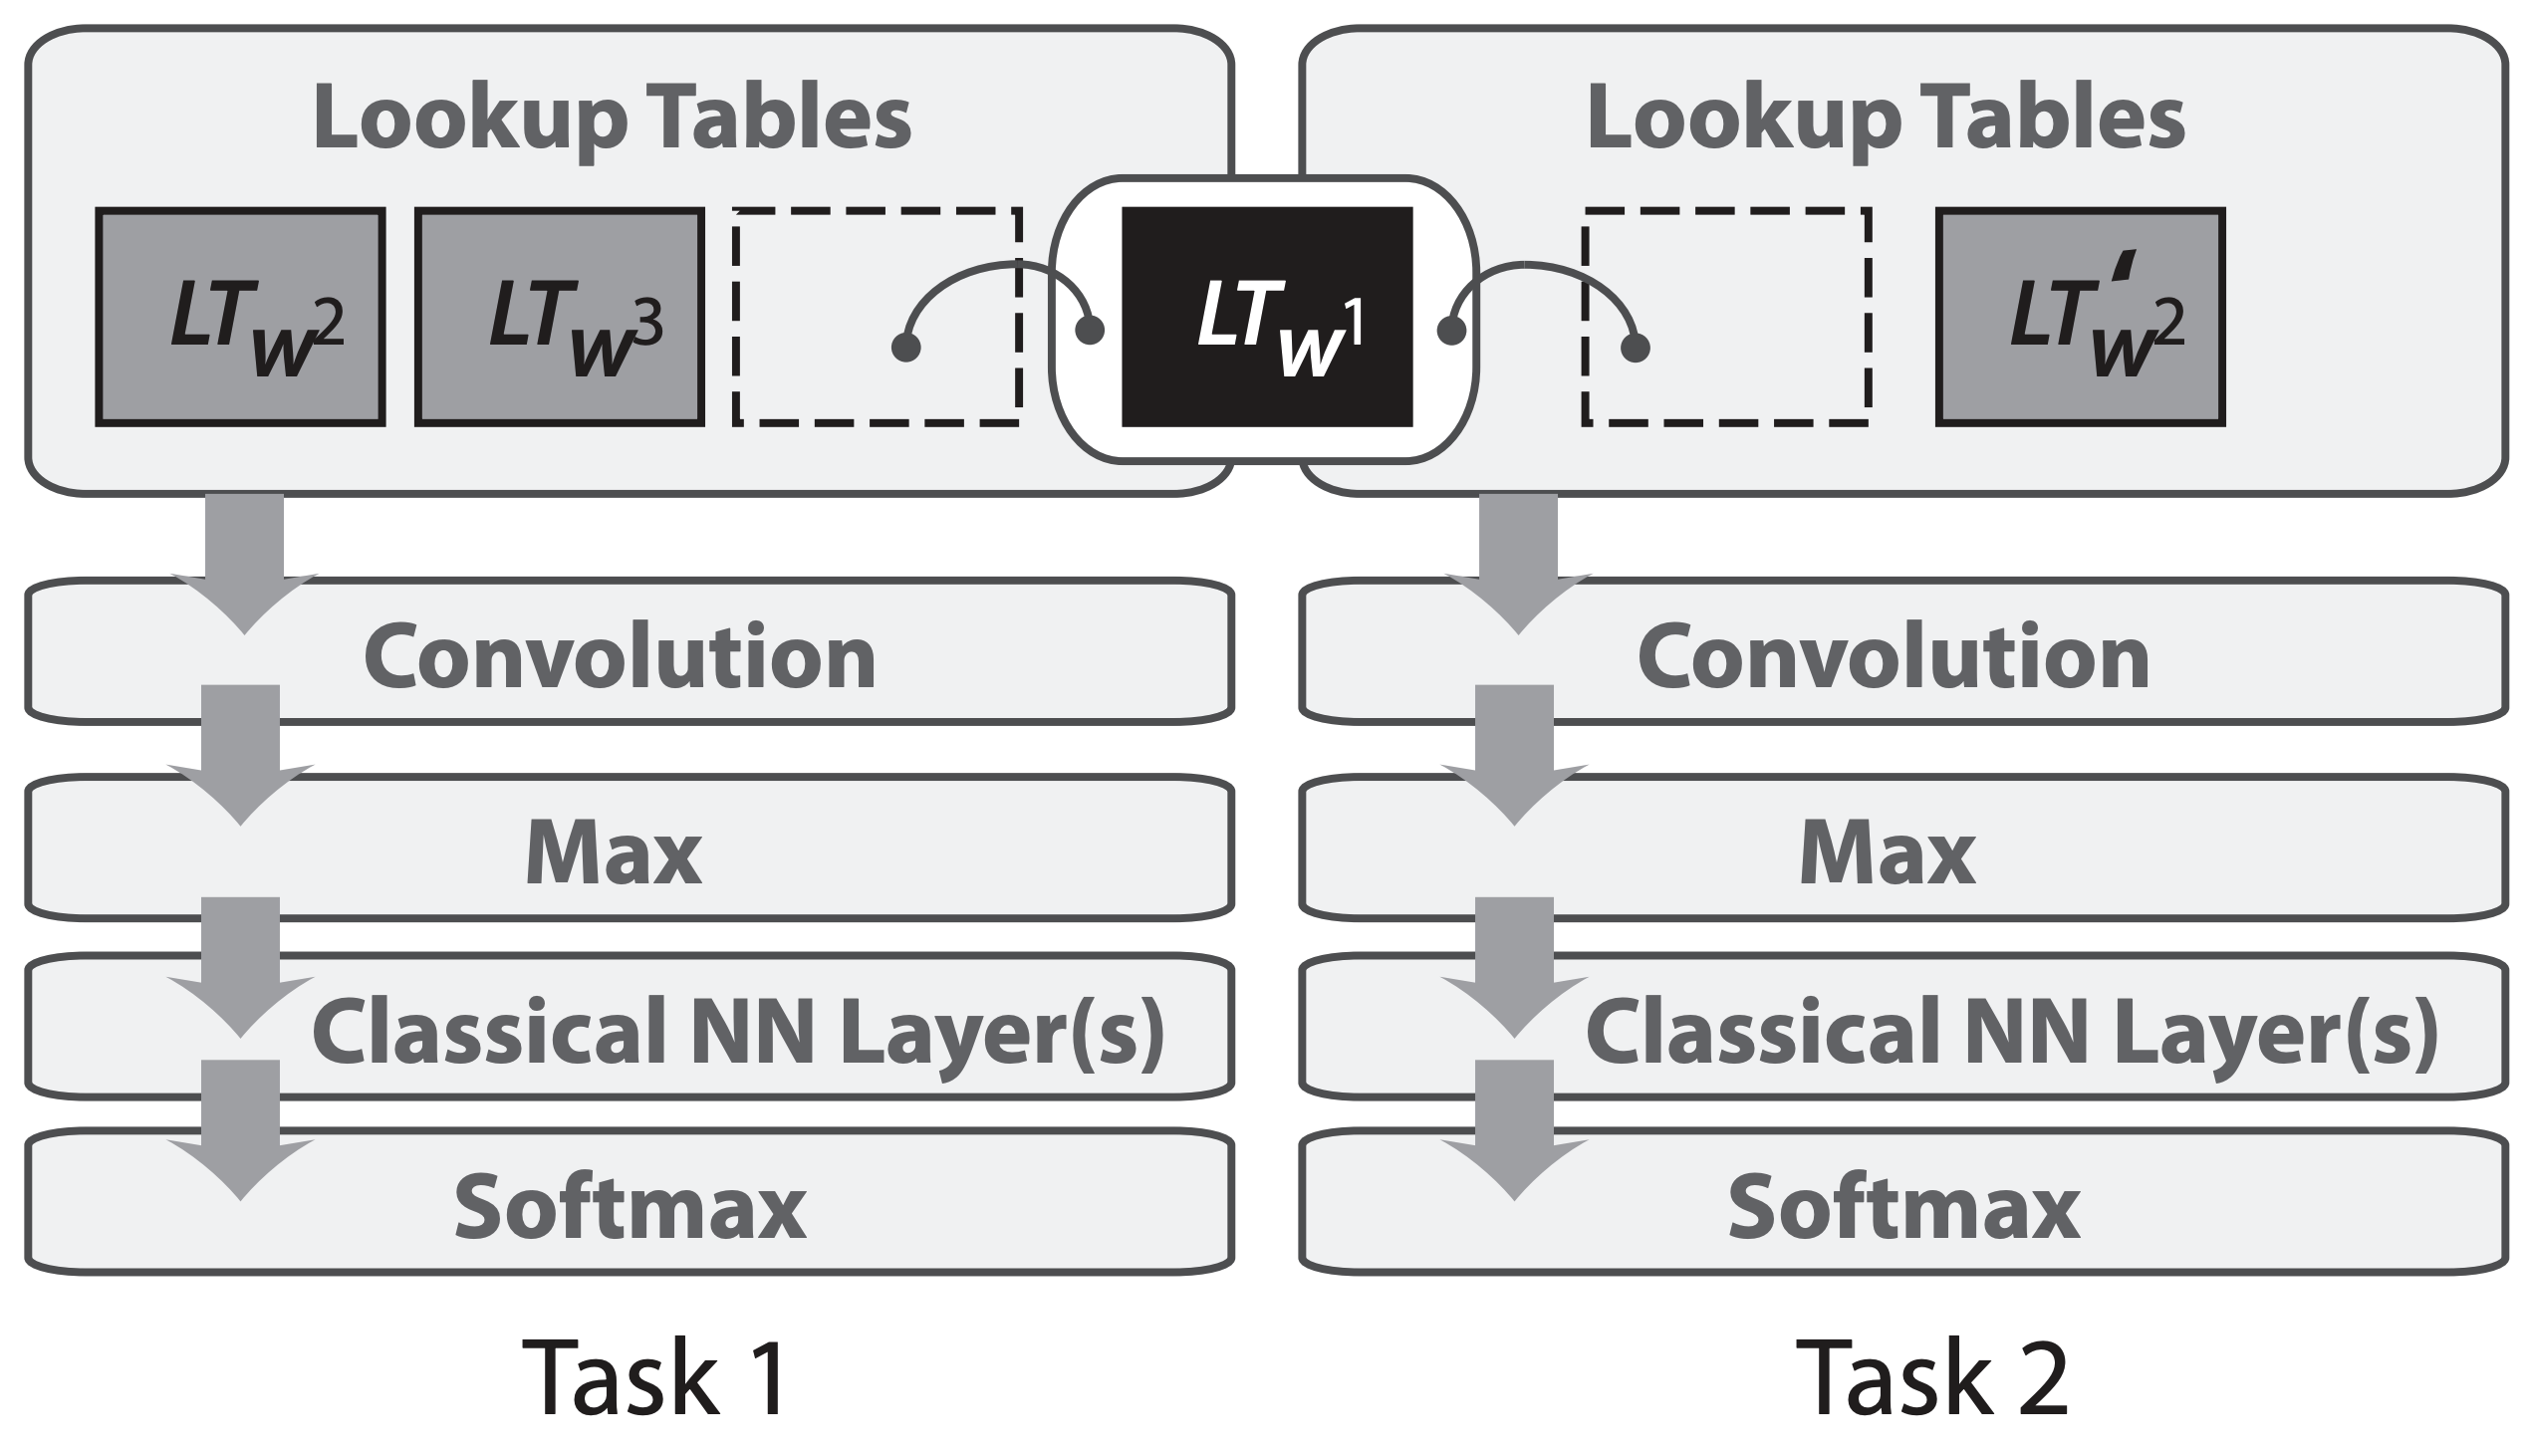
\includegraphics[scale=0.2]{imgs/sharing.png}
      \end{center}
      
  \end{frame}


  \section{Leveraging Unlabeled Data}
  \begin{frame}{Leveraging Unlabeled Data}
      \begin{itemize}[<+->]
          \item Labeling is expensive.
          \item Leveraging unlabeled data in NLP seems like a good idea.
              \pause{\color{gray}10 years later this still rings true.}
      \end{itemize}
      
  \end{frame}

  \begin{frame}{Leveraging Unlabeled Data - Language Model}
      \begin{itemize}[<+->]
          \item $2$-class classification task: Predict whether the middle word
              of a window is related to its context or not.
          \item Training dataset was built from Wikipedia. Positive examples are
              real extracts from Wikipedia, negative ones are the same ones but
              with the middle word replaced by a random one.
          \item Ranking-type (hinge) loss:
              $$\sum_{s\in\mathcal{S}}\sum_{w\in\mathcal{D}}\max(0,1-f(s)+f(s^w))$$
              $\mathcal{S}$ is the set of sentence windows, and $\mathcal{D}$ the
              set of words in the vocabulary.
      \end{itemize}
  \end{frame}

  \begin{frame}{Leveraging Unlabeled Data - Language Model}
      Word representations learned by this model cluster for semantically-similar
      words. In other words, the embedding space learned by this model encodes
      semantic similarity.
      \begin{center}
        \pause[\thebeamerpauses]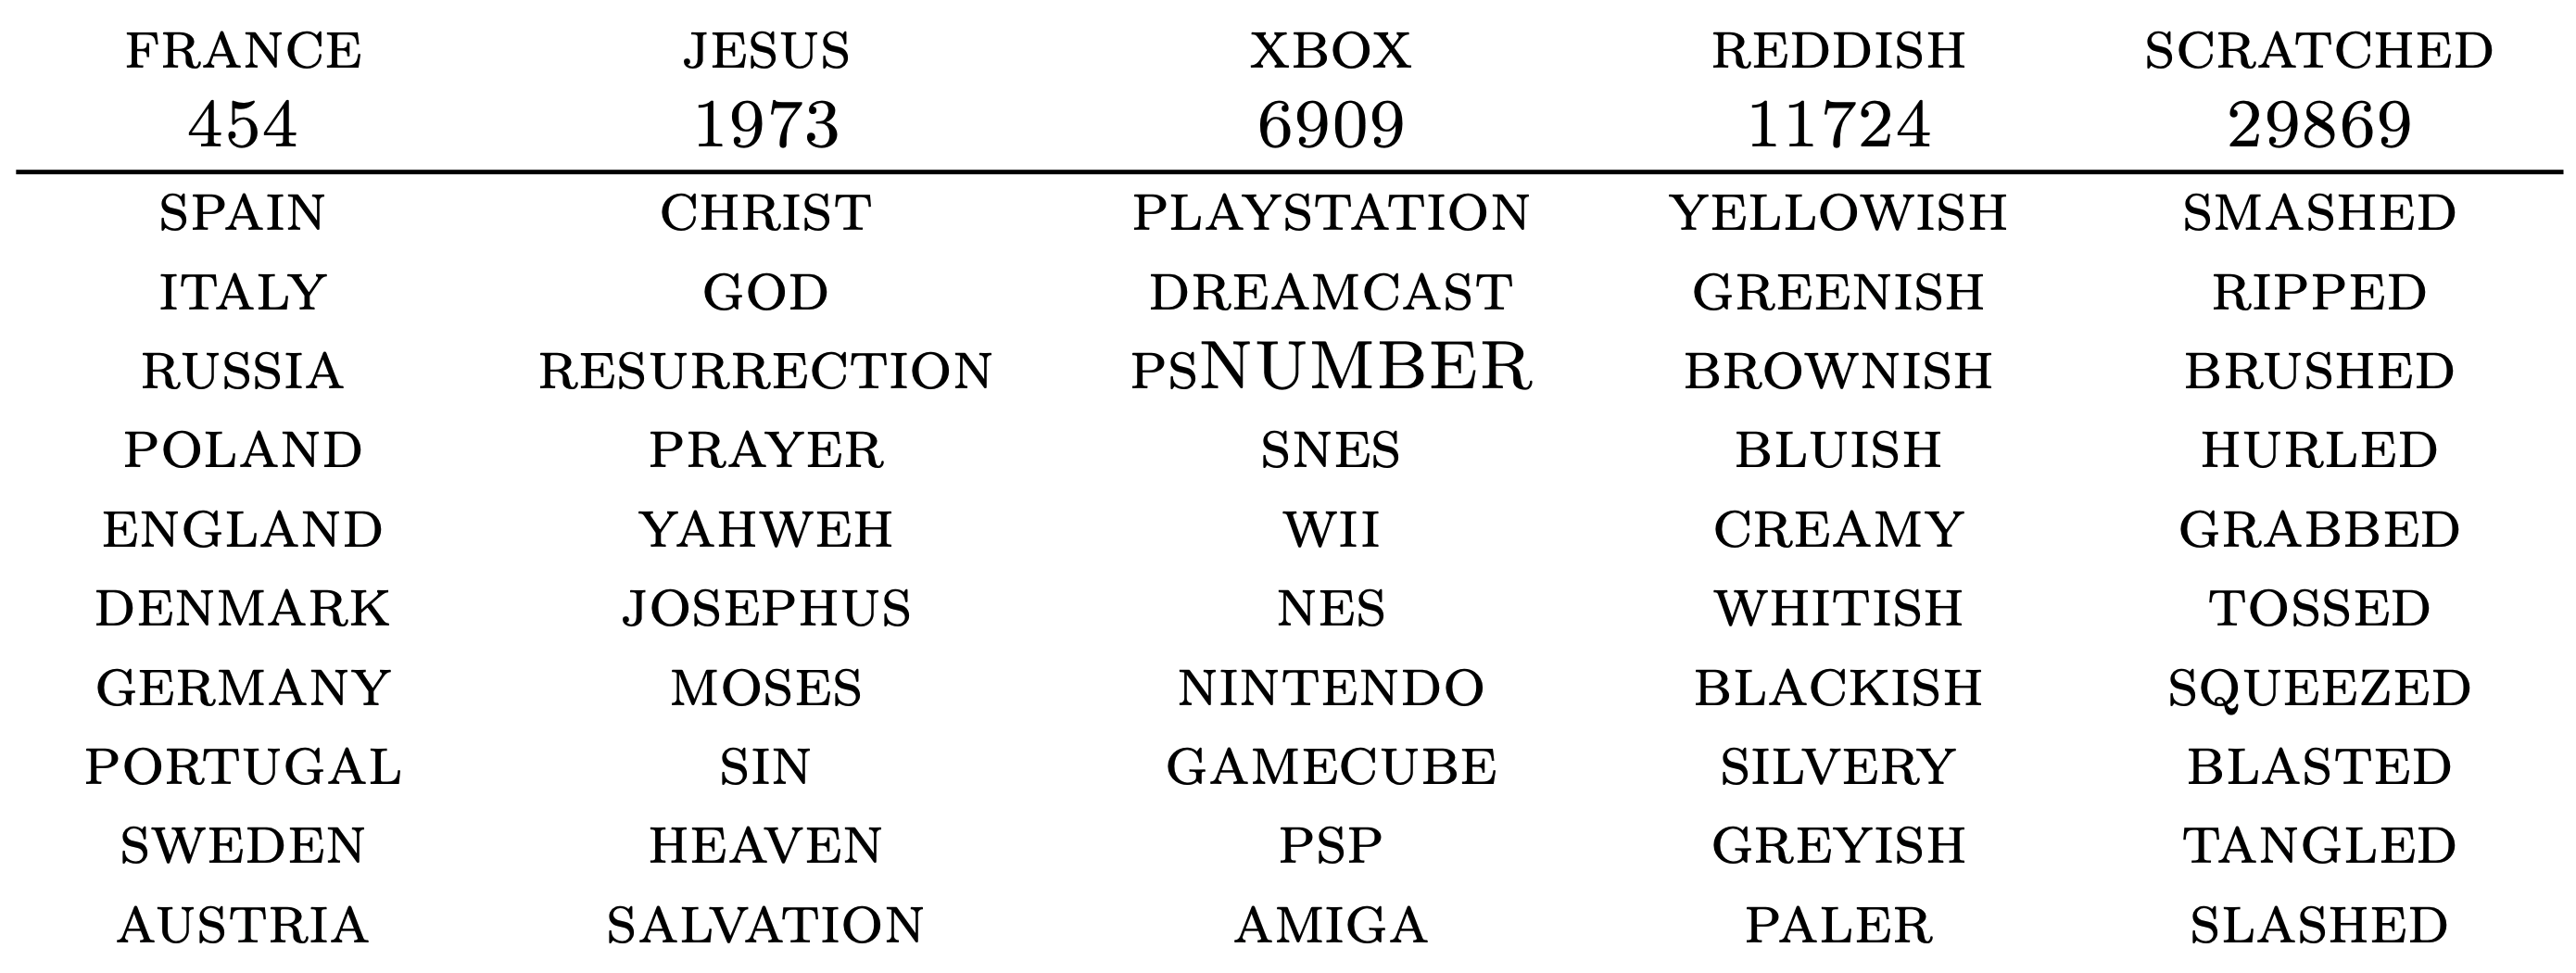
\includegraphics[scale=0.2]{imgs/wordsim.png}
      \end{center}
  \end{frame}

  \section{Experiments}
  \begin{frame}{Experiments - Results}
      \hspace{-0.5cm}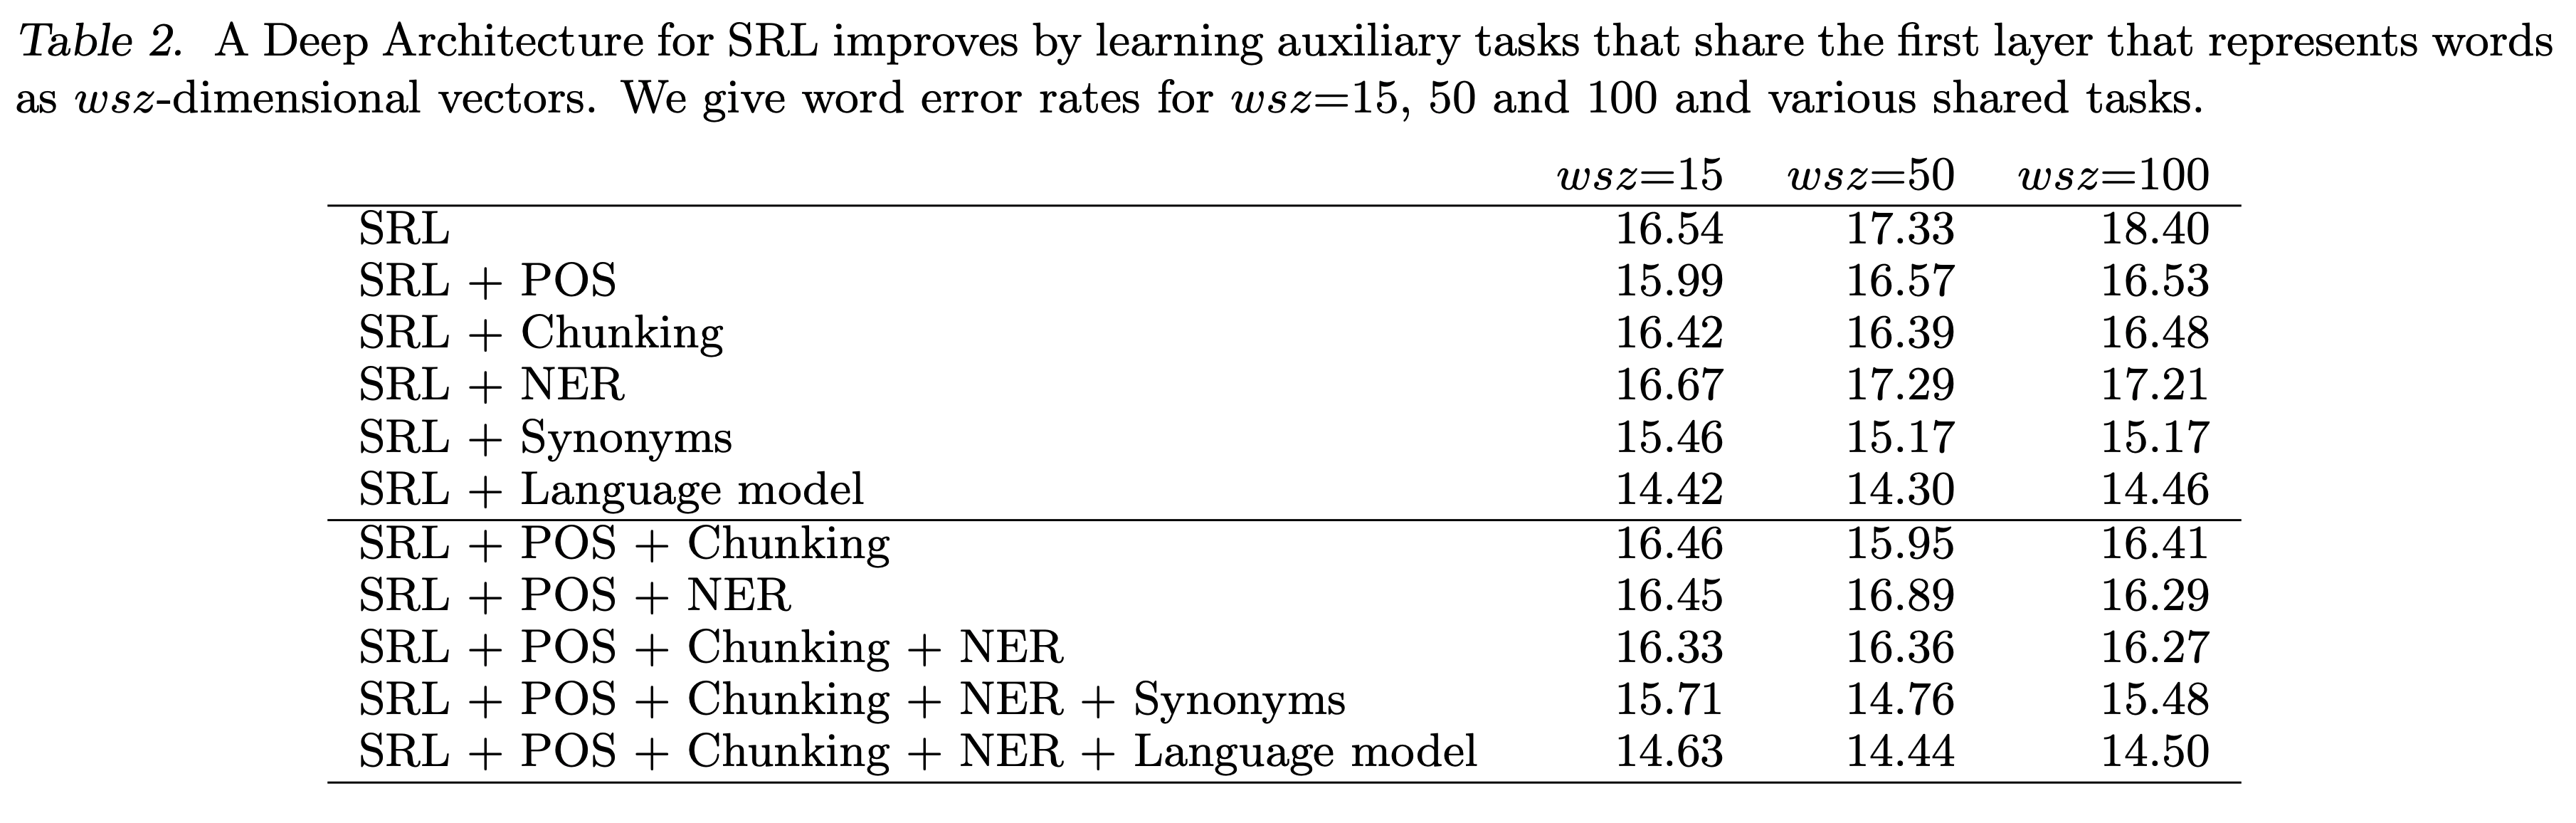
\includegraphics[scale=0.18]{imgs/results.png}
  \end{frame}
  \begin{frame}{Experiments - Results}
      \hspace{-0.6cm}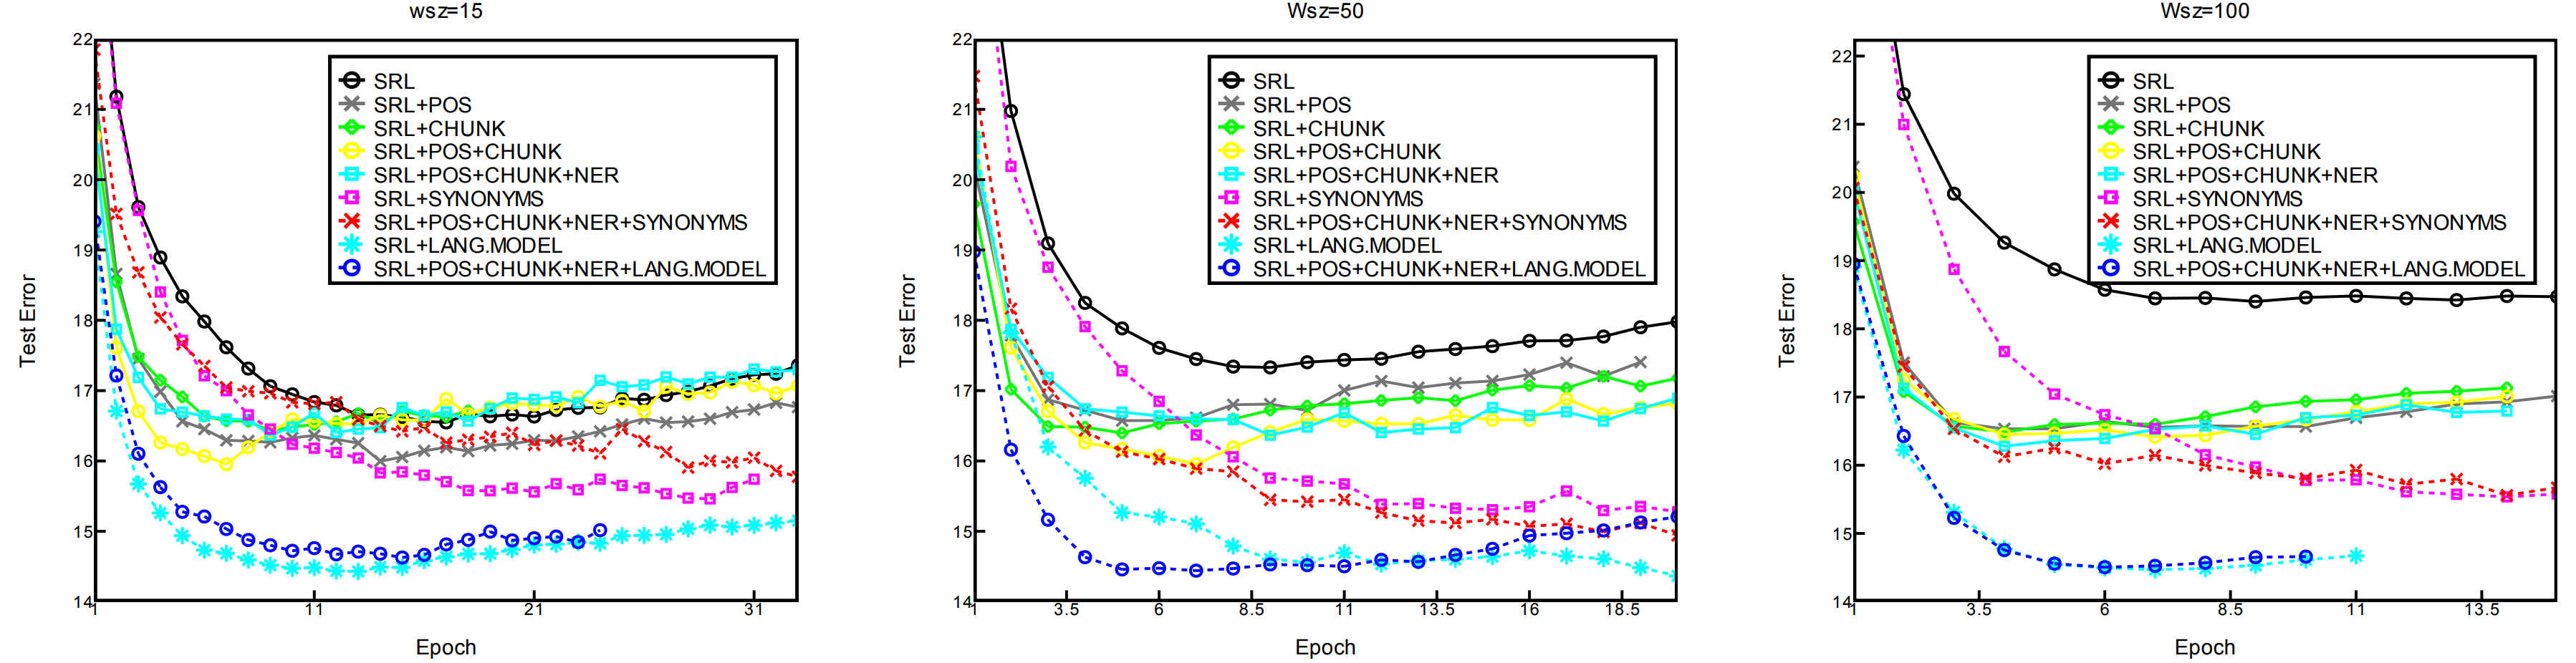
\includegraphics[scale=0.18]{imgs/resultgraphs.png}
  \end{frame}
  \section{Conclusion}
  \begin{frame}{Conclusion}
      \begin{itemize}
          \item They showed a deep NN for NLP.
          \item Architecture is extremely fast.
          \item Architecture can be applied to several tasks.
          \item \textbf{Learning tasks simultaneously improved generalization
                  performance.}
          \item Achieved state of the art in SRL when training this task jointly
              with their language model \textit{without any explicit syntactic
              features}.
      \end{itemize}
  \end{frame}

  \section{Discussion}

\bibliographystyle{emnlp_natbib}
\bibliography{bibliography}
\end{document}
